% main.tex -- IEEE conference paper covering both prefetching studies in
% this repository (disk blocks: src/adaptive_prefetch; product pages:
% src/webprefetch). Compile on Overleaf with pdfLaTeX + BibTeX; no local
% LaTeX toolchain is available (MASTER_PLAN L6). `python paper/check.py`
% is the local gate. See paper/README.md.
%
% Rules for everything under sections/ (enforced by check.py):
%   - Every number quoted in prose is a macro from numbers.tex, which
%     paper/numbers.py writes from results/. Nothing is typed by hand.
%   - Tables come from tables/*.tex (paper/tables/make_tables.py) and
%     figures from figures/*.pdf (paper/figures/make_figures.py). Both read
%     only results/**.
%   - Every \cite key exists in refs.bib.

\documentclass[conference]{IEEEtran}
\IEEEoverridecommandlockouts

\usepackage{cite}
\usepackage{amsmath,amssymb}
\usepackage{graphicx}
\usepackage{url}
\usepackage{xcolor}

% Generated: one \newcommand per quoted number (WP13 writes it). The guard
% lets the skeleton compile on Overleaf before numbers.tex exists; once the
% prose uses a macro, a missing numbers.tex is an undefined-command error,
% and `check.py --strict` already fails on it.
\IfFileExists{numbers.tex}{% numbers.tex -- GENERATED by paper/numbers.py from results.
% Do not edit: rerun `python reproduce.py paper`. Every number the prose
% quotes is one of these macros (MASTER_PLAN section 5; paper/check.py).
% MISSING input: disk/corpus_profile.csv
% MISSING input: disk/deltas.csv
% MISSING input: disk/kappa.csv
% MISSING input: disk/table_by_corpus.csv
% MISSING input: disk/table_main.csv
% MISSING input: gpu/disk_learned_depth.csv
% MISSING input: live/live_metrics.csv
% MISSING input: live/live_parity.csv
% MISSING input: realio/realio_summary.csv
% MISSING input: web/comparisons.csv
% MISSING input: web/dataset_profile.json
% MISSING input: web/decomposition.csv
% MISSING input: web/freshness.csv
% MISSING input: web/policy_metrics.csv
% MISSING input: web/seq_metrics.csv
\providecommand{\missingnumber}{\textbf{??}}
\providecommand{\fixturemark}[1]{\textcolor{red}{#1\textsuperscript{FIXTURE}}}
\providecommand{\paperFixtureData}{false}
% --- disk/corpus_profile.csv
\newcommand{\diskCorpora}{\missingnumber}
\newcommand{\diskTraces}{\missingnumber}
% --- disk/deltas.csv
\newcommand{\diskAdaptiveVsSeq}{\missingnumber}
\newcommand{\diskAdaptiveVsSeqCI}{\missingnumber}
\newcommand{\diskAdaptiveVsSeqHi}{\missingnumber}
\newcommand{\diskAdaptiveVsSeqLo}{\missingnumber}
\newcommand{\diskAdaptiveVsSeqLosses}{\missingnumber}
\newcommand{\diskAdaptiveVsSeqN}{\missingnumber}
\newcommand{\diskAdaptiveVsSeqWins}{\missingnumber}
\newcommand{\diskDeepEightIORatio}{\missingnumber}
\newcommand{\diskDeepEightIORatioCI}{\missingnumber}
\newcommand{\diskDeepEightIORatioHi}{\missingnumber}
\newcommand{\diskDeepEightIORatioLo}{\missingnumber}
\newcommand{\diskDeepEightIORatioLosses}{\missingnumber}
\newcommand{\diskDeepEightIORatioN}{\missingnumber}
\newcommand{\diskDeepEightIORatioWins}{\missingnumber}
\newcommand{\diskDeepEightVsNone}{\missingnumber}
\newcommand{\diskDeepEightVsNoneCI}{\missingnumber}
\newcommand{\diskDeepEightVsNoneHi}{\missingnumber}
\newcommand{\diskDeepEightVsNoneLo}{\missingnumber}
\newcommand{\diskDeepEightVsNoneLosses}{\missingnumber}
\newcommand{\diskDeepEightVsNoneN}{\missingnumber}
\newcommand{\diskDeepEightVsNoneWins}{\missingnumber}
\newcommand{\diskGuardVsSeq}{\missingnumber}
\newcommand{\diskGuardVsSeqCI}{\missingnumber}
\newcommand{\diskGuardVsSeqHi}{\missingnumber}
\newcommand{\diskGuardVsSeqLo}{\missingnumber}
\newcommand{\diskGuardVsSeqLosses}{\missingnumber}
\newcommand{\diskGuardVsSeqN}{\missingnumber}
\newcommand{\diskGuardVsSeqWins}{\missingnumber}
\newcommand{\diskLinuxRaIORatio}{\missingnumber}
\newcommand{\diskLinuxRaIORatioCI}{\missingnumber}
\newcommand{\diskLinuxRaIORatioHi}{\missingnumber}
\newcommand{\diskLinuxRaIORatioLo}{\missingnumber}
\newcommand{\diskLinuxRaIORatioLosses}{\missingnumber}
\newcommand{\diskLinuxRaIORatioN}{\missingnumber}
\newcommand{\diskLinuxRaIORatioWins}{\missingnumber}
\newcommand{\diskLinuxRaVsNone}{\missingnumber}
\newcommand{\diskLinuxRaVsNoneCI}{\missingnumber}
\newcommand{\diskLinuxRaVsNoneHi}{\missingnumber}
\newcommand{\diskLinuxRaVsNoneLo}{\missingnumber}
\newcommand{\diskLinuxRaVsNoneLosses}{\missingnumber}
\newcommand{\diskLinuxRaVsNoneN}{\missingnumber}
\newcommand{\diskLinuxRaVsNoneWins}{\missingnumber}
% --- gpu/disk_learned_depth.csv
\newcommand{\ldVsVcf}{\missingnumber}
\newcommand{\ldVsVcfCI}{\missingnumber}
\newcommand{\ldVsVcfHi}{\missingnumber}
\newcommand{\ldVsVcfLo}{\missingnumber}
\newcommand{\ldVsVcfLosses}{\missingnumber}
\newcommand{\ldVsVcfN}{\missingnumber}
\newcommand{\ldVsVcfWins}{\missingnumber}
% --- live/live_metrics.csv
\newcommand{\liveInvalidPasses}{\missingnumber}
% --- live/live_parity.csv
\newcommand{\liveParityMismatches}{\missingnumber}
% --- prefetch_common.utility
\newcommand{\diskAssumedC}{$0.526$}
\newcommand{\diskBreakEvenC}{$1.0101$}
% --- web/comparisons.csv
\newcommand{\webControllerVsBestFixed}{\missingnumber}
\newcommand{\webControllerVsBestFixedCI}{\missingnumber}
\newcommand{\webControllerVsBestFixedHi}{\missingnumber}
\newcommand{\webControllerVsBestFixedLo}{\missingnumber}
% --- web/decomposition.csv
\newcommand{\webFreshnessLever}{\missingnumber}
\newcommand{\webFreshnessLeverCI}{\missingnumber}
\newcommand{\webFreshnessLeverHi}{\missingnumber}
\newcommand{\webFreshnessLeverLo}{\missingnumber}
}{%
  \typeout{numbers.tex has not been generated; run python reproduce.py paper}}

% The validated web controllers, by the names results/web/comparisons.csv
% gives them (capacity 8, the pre-registered cost), so no policy parameter is
% typed into the prose. E6 replays exactly these three.
\newcommand{\polAdaptive}{\texttt{\webCmpAdaptivePolicyPerCapacityLogisticCapEightCostZeroPointZeroOne}}
\newcommand{\polFeedback}{\texttt{\webCmpAdaptivePolicyPerCapacityLogisticFeedbackCapEightCostZeroPointZeroOne}}
\newcommand{\polOnline}{\texttt{\webCmpAdaptivePolicyPerCapacityTransOnlineCapEightCostZeroPointZeroOne{}@trans\_online}}

% Skeleton marker for unwritten text. `check.py --final` fails while any
% \todo remains, so none can reach the submitted paper.
\newcommand{\todo}[1]{\textcolor{red}{[TODO: #1]}}

\begin{document}

% Title (WP14), chosen from how the pre-registered comparisons came out
% (paper/decisions.py, tables/t9_decisions.tex). The working title of MASTER_PLAN section 5
% ("Depth, Freshness and Feedback, Not Prediction") is contradicted on two
% counts: the feedback gate never beat its baseline in either study, and
% neither study's rule calls the learned predictor the *smallest* lever. What
% the rules do support is that every learned predictor lost to its simple
% fair baseline while depth (or window growth) and freshness moved the
% simulated hit ratio, and that simulated hit ratio did not rank measured
% latency on the real disk.
\title{Depth and Freshness, Not Learned Prediction:\\
A Pre-Registered Study of Prefetching from Disk Blocks to Product Pages}

% Students only; no supervisor or other author is listed.
% E-mail addresses are left out on purpose; add them here before submission:
% \IEEEauthorblockA{... \\ <e-mail>}
\author{%
\IEEEauthorblockN{Ashvik Mishra (24BAI0342)}
\IEEEauthorblockA{School of Computer Science and Engineering\\
Vellore Institute of Technology\\
Vellore, India}
\and
\IEEEauthorblockN{Shourya Saraf (24BDS0391)}
\IEEEauthorblockA{School of Computer Science and Engineering\\
Vellore Institute of Technology\\
Vellore, India}
}

\maketitle

% Abstract and index terms. Written from the outcome of the pre-registered
% comparisons (paper/decisions.py; tables/t9_decisions.tex); every number is a numbers.tex
% macro. Five claims: disk sweep, real device, web decomposition, live HTTP,
% and the classifier study (pre-registered after the first four were known).

\begin{abstract}
Kernels and browsers both prefetch. We ask which decision moves the result,
under rules fixed before the experiments ran. \emph{Disk (simulated):} on \diskTraces{} block
traces from \diskCorpora{} corpora and a 1\,MiB cache, a learned workload-class
router hit less often than plain sequential read-ahead
(\decDiskPOneAdaptiveAssumedOneMiBPairedCI) with \diskIORatioAdaptiveOneMiB{} the
device I/Os of no prefetching, and a GPU-trained depth controller
less often than a validation-chosen fixed depth
(\decDiskLearnedDepthVsVcfCapTwoHundredFiftySixPairedCI), while Linux-style
window growth added \decDiskPFourLinuxRaAtTwoHundredFiftySixAssumedOneMiBPaired{}
and cut device I/Os to \decDiskPFiveLinuxRaAtTwoHundredFiftySixOneMiBPaired{} of no
prefetching's.
\emph{Real devices (measured):} on a hard disk and an SSD, the mode with the highest simulated hit ratio was fastest in
\decCellsTopSimFastest{} of \decCells{} cells, and with exact cache parity
prefetching raised the mean closed-loop latency on the hard disk in
\decCountROneSdbOdirectClosedRaises{} of \decCountROneSdbOdirectClosed{}
mode--trace cells.
\emph{Web (simulated):} on RetailRocket, transition counts beat a trained
ranker (\decWebWThreeHitRankerCI), online counts beat a GRU
(\decWebWEightHitSequenceModelCI), and index freshness gave
\decWebWFourHitFreshnessCI.
\emph{Live HTTP (measured, emulated network):} every prefetching policy
lowered the wait with a hard-disk store, by up to
\liveSavedHddAdaptiveZeroPointOneAtTransOnline{} per view against
\liveBaseWaitHdd{} without prefetching, with exact simulator parity.
\emph{Better learners (simulated):} none of \clfRouterClassifiers{}
classifiers made the router beat sequential read-ahead, a hindsight-trained
router choosing depth did not beat a per-trace fixed depth, and a tuned web
ranker gained \decWrkSOneMlpUtilityPerViewCapEight{} in utility but stayed
below transition counts.
How much to fetch and how fresh the statistics are moved the results; no
learned predictor beat its simple baseline, and simulated hit ratio did not
predict real-disk latency.
\end{abstract}

\begin{IEEEkeywords}
prefetching, read-ahead, page cache, storage traces, web prefetching,
cache simulation, machine learning for systems, pre-registration
\end{IEEEkeywords}


% I. Introduction. No results file: this section motivates and lists the
% contributions. Numbers that appear in the contribution list are macros.

\section{Introduction}\label{sec:intro}

\todo{The operating-system problem: page-cache read-ahead in the kernel and
browser or proxy prefetch on the web both spend device or network work now
to hide latency later, and both must decide what and how much to fetch.}

\todo{Why learning is the obvious answer and why the question is whether it
is the lever that matters. State the thesis as the hypothesis tested by the
preregistered comparisons in results/disk/PREREGISTERED.md,
results/web/PREREGISTERED.md and results/live/PREREGISTERED.md, not as a
foregone conclusion.}

\todo{Contributions, as a bulleted list: the multi-corpus negative result
for the learned class router; depth versus device-I/O decoupling; a real
Linux testbed with exact simulator parity; the web freshness and controller
decomposition; and the live HTTP replay.}

\todo{Roadmap of the remaining sections.}

% II. Background and related work. Every key cited below is in refs.bib and
% was verified (docs/REFERENCES.md). Uses the corrected titles and venues for
% CAPSULE, Savva and Herodotou, Akgun et al. and the ECML PKDD chapter; the
% NVMW'22 abstract is non-archival and is cited as such.

\section{Background and Related Work}\label{sec:related}

\textbf{Read-ahead in the kernel.} Linux keeps a per-file read-ahead window
that grows while the reader stays sequential and collapses on a random
access; a marker page triggers the next asynchronous
batch~\cite{wu2007readahead,wu2010concurrent,linux_mmapi_readahead}, and
applications can add hints~\cite{man_posix_fadvise,man_readahead}. Our
\texttt{linux\_ra} emulates this window; the testbed measures the kernel's
own.

\textbf{Prefetching in storage caches.} Sequential prefetching with adaptive
degree and trigger distance is standard in storage
controllers~\cite{gill2005sarc,gill2007amp}; other work exploits disk layout
and access history~\cite{ding2007diskseen}, mined block
correlations~\cite{li2004cminer} or server-side
context~\cite{soundararajan2008context}. Informed prefetching uses application
hints and bounds how far ahead to fetch~\cite{patterson1995informed}, and
integrated prefetching and caching studies when a prefetch should replace a
cached block~\cite{cao1995integrated}. Predictive file prefetching goes back to
probability graphs and Markov predictors~\cite{griffioen1994reducing,
kroeger2001design,joseph1997markov}.

\textbf{Learned prefetching.} LSTM models of address
deltas~\cite{hochreiter1997lstm,hashemi2018learning} have been applied to SSD
traces~\cite{chakraborttii2020learning} and to flash (a non-archival
workshop abstract~\cite{chakraborttii2022deep}). Online and streaming learners
adapt file-system prefetching as the workload
changes~\cite{savva2026adaptive,lucasfilho2023streaming}. Baleen learns
admission and prefetch for flash caches~\cite{wong2024baleen}, CAPSULE clusters
spatio-temporal locality for cloud block storage~\cite{ramadhan2026capsule},
KML runs models inside the kernel~\cite{akgun2021kml}, and CrossPrefetch
coordinates prefetching across the OS and the library~\cite{garg2024crossprefetch}.
Memory-side work learns remote-memory prefetch and page
placement~\cite{maruf2020leap,doudali2019kleio}. Such work usually compares a
learned model with one heuristic on a few traces; we fix the simple baselines
in advance and measure the other levers on the same traces.

\textbf{Reference points from cache theory.} Belady's MIN is the optimal
demand-paging replacement~\cite{belady1966study}; it does not bound a policy
that prefetches, and we never use it as such a bound. Stack-distance
analysis~\cite{mattson1970evaluation} is the classical evaluation tool, and
adaptive, FIFO-based and learned
eviction~\cite{megiddo2003arc,yang2023fifo,zhang2024sieve,yang2023glcache,
shi2019glider} change the replacement policy; we keep LRU fixed so that only
prefetching varies.

\textbf{Web prefetching and next-item models.} Predictive prefetching of web
pages~\cite{padmanabhan1996using}, its latency bounds~\cite{kroeger1997exploring}
and its cost over slow links~\cite{fan1999web} raised the same what and
how-much questions in the 1990s. Session-based next-item models range from
GRUs to self-attention~\cite{hidasi2016session,kang2018sasrec}; we test a GRU
as a ranker.

We do not propose a predictor; we measure, under pre-registered rules,
which lever moves the outcome, and check the simulators against a real disk
and real HTTP.

% III. A common model of prefetching. Definitions only; no measured
% numbers. The derivation of the disk break-even must say it is a property
% of the per-block, no-merge cost model, not of hardware (constraint 6).
% Feeds from: docs/METRICS.md, src/prefetch_common/utility.py.
% Figure F1 (schematic) comes from paper/figures/make_figures.py.
% If space is short, fold this section into Sections IV-A and IV-C.

\section{A Common Model of Prefetching}\label{sec:model}

\todo{The cache abstraction shared by both domains: a demand stream, a
bounded LRU cache, and a policy that issues speculative fetches.}

\todo{Definitions from docs/METRICS.md: block hit ratio per 512-byte block,
device I/Os, prefetch precision, wasted prefetches and cache pollution.}

\todo{The utility U(c) = (hits - c * issued) / requests, the derivation of
the disk cost model as U at c = p m / (m - h), the per-policy break-even
c*, and kappa* (from src/prefetch\_common/utility.py). Quote the disk
break-even only through its numbers.tex macro.}

\todo{Fig. F1: the schematic of the shared abstraction.}

% IV. Systems. Describes code, not results. Kernel facts quoted here are
% cited to the man pages and kernel documentation in refs.bib section G.
% Feeds from: src/adaptive_prefetch (WP3), src/adaptive_prefetch/realio
% (WP8), src/webprefetch (WP5), src/webprefetch/live (WP12).

\section{Systems}\label{sec:systems}

\subsection{Disk simulator and policies}\label{sec:systems-disk}
\todo{The causal replay loop shared by every mode, the first-window
prefetch gate, the twelve modes plus linux\_ra and learned\_depth, and
the device-I/O accounting (WP3).}

\subsection{Real Linux testbed}\label{sec:systems-realio}
\todo{Backend A: buffered reads through the page cache with
POSIX\_FADV\_WILLNEED hints~\cite{man_posix_fadvise} inside a memory
cgroup~\cite{linux_cgroup_v2}. Backend B: O\_DIRECT~\cite{man_open} reads
with asynchronous prefetch threads. The online driver. Kernel facts: the
per-call WILLNEED truncation, the cgroup charging rule, and residency
checks with cachestat versus RWF\_NOWAIT~\cite{man_cachestat,man_readv};
the host kernel uses the multi-gen LRU~\cite{linux_mglru} (WP8).}

\subsection{Web replay}\label{sec:systems-web}
\todo{Per-session LRU cache, the ranker and its scorers, the fixed and
adaptive controllers, the online index, and the feedback gate (WP5).}

\subsection{Live HTTP replay}\label{sec:systems-live}
\todo{The asyncio origin, the precise timer, the priority link and the
validity gate (WP12).}

% V. Methodology. Every count, cap and hardware figure comes from the
% results files below through numbers.tex or a generated table.
% Feeds from: results/disk/corpus_profile.csv, results/web/dataset_profile.json,
% results/realio/device_*.json, results/gpu/gpu_env.json, and the
% provenance.json in each results directory.
% Table T1 (datasets) comes from paper/tables/make_tables.py.

\section{Methodology}\label{sec:method}

\todo{Table T1 (datasets): the oracleGeneral block traces in four corpora
with their reconstruction rules (MSR, Alibaba and Tencent records as
requests; FIU pages merged into requests with a sector cap), twin traces
and request caps, from results/disk/corpus\_profile.csv; and the
RetailRocket splits from results/web/dataset\_profile.json. Cite the trace
and dataset sources~\cite{narayanan2008write,koller2010iodedup,
li2020alibaba,zhang2020osca,snia_tencent_cbs,cmupdl_cachedatasets,
yang2020twemcache,libcachesim,retailrocket2017}.}

\todo{Protocols: chronological validation and test splits; paired and
cluster bootstrap CIs (method, resamples and seed from the PREREGISTERED.md
files); repeats per configuration; the training range of every trained
artifact, which is never scored on its own training segment.}

\todo{Hardware table: CPU, the HDD and SSD models, kernel, page-cache
reclaim policy, and the GPU with its contention record, from
results/realio/device\_*.json and results/gpu/gpu\_env.json. Software:
PyTorch~\cite{paszke2019pytorch} and
scikit-learn~\cite{pedregosa2011sklearn}.}

% VI. Disk results (simulated). Every number is a simulated block hit ratio
% of an LRU cache on canonical requests (constraints 1, 13); writes replay as
% reads, and nothing is compared numerically with the MSRC-trace-003 (D17)
% numbers (constraint 5). Hit ratio is always paired with device work (lead
% ruling); belady_min is demand-only MIN, not a bound on prefetching.
% Sources: results/disk/{table_main,table_by_corpus,deltas,kappa}.csv (E1),
% results/gpu/{disk_learned_depth,disk_lstm}.csv (E2), via numbers.tex and
% paper/decisions.py. Generated: Table T2; Fig. F3 (F2, F4, T2b, T2c in the
% appendix).

\section{Disk Results (Simulated)}\label{sec:disk}

% t2_disk_main.tex -- GENERATED by paper/tables/make_tables.py; do not edit.
% Inputs: none
% MISSING input: disk/table_main.csv
\begin{table*}[t]
\centering
\footnotesize
\setlength{\tabcolsep}{3pt}
\caption{Disk results (simulated LRU cache, C1 configuration, canonical requests). Mean block hit ratio over traces; $\Delta$ in percentage points with 95\% paired-bootstrap CIs over traces; device-I/O and blocks-moved ratios are means over traces of the policy's count over \texttt{none}'s. $^\dagger$ gated mode at the break-even cost model. Writes replay as reads.}
\label{tab:t2_disk_main}
\begin{tabular}{l}
\hline
\textbf{MISSING: disk/table\_main.csv} \\
\hline
\end{tabular}
\end{table*}


All numbers in this section are simulated block hit ratios
(Table~\ref{tab:t2_disk_main}).

\textbf{How much to prefetch.} This is the largest lever (P3, P4). Fixed
read-ahead (\texttt{deep@8}) is \decDiskPThreeDeepAtEightAssumedOneMiBVerdict{}
than no prefetching at both capacities
(\decDiskPThreeDeepAtEightAssumedOneMiBPairedCI{} paired and
\decDiskPThreeDeepAtEightAssumedOneMiBClusterCI{} cluster at 1\,MiB, winning on
\diskDeltaHitRatioDeepAtEightVsNoneOneMiBWins{} of \diskDeltaHitRatioDeepAtEightVsNoneOneMiBN{}
traces). In the C2 depth sweep the deepest depth tested
(\diskCTwoDeepest{} blocks) has the highest mean hit ratio in
\diskCTwoBestIsDeepest{} of the \diskCTwoCurves{} corpus--cache curves; only at
1\,MiB do Alibaba and MSR peak earlier, at \diskCTwoBestDepthAlibabaOneMiB{} and
\diskCTwoBestDepthMsrOneMiB{} blocks (Fig.~\ref{fig:f2} in the appendix). In C1,
\texttt{deep@256} adds
\decDiskPThreeDeepAtTwoHundredFiftySixAssumedOneMiBPaired{} at 1\,MiB and
\decDiskPThreeDeepAtTwoHundredFiftySixAssumedSixtyFourMiBPaired{} at 64\,MiB.
Linux-style window growth gets much of that gain with far less waste:
\texttt{linux\_ra@256} adds \decDiskPFourLinuxRaAtTwoHundredFiftySixAssumedOneMiBPairedCI{}
at 1\,MiB, wins on all \diskDeltaHitRatioLinuxRaAtTwoHundredFiftySixVsNoneOneMiBN{}
traces, and leaves \diskWasteLinuxRaAtTwoHundredFiftySixOneMiB{} of its prefetches
unused, against \diskWasteDeepAtTwoHundredFiftySixOneMiB{} for \texttt{deep@256}.
Belady's MIN for demand paging reaches \diskHitBeladyMinOneMiB{} at 1\,MiB
(\texttt{none}: \diskHitNoneOneMiB); several prefetching policies exceed it,
as they may: MIN bounds replacement, not prefetching.

\textbf{Hit ratio is not device work} (P5, P6; Fig.~\ref{fig:f3}). At
1\,MiB, \texttt{deep@8}
\decDiskPFiveDeepAtEightOneMiBVerdict{}
(\decDiskPFiveDeepAtEightOneMiBPairedCI{} of \texttt{none}'s), and
\texttt{deep@256} moves \diskMovedRatioDeepAtTwoHundredFiftySixOneMiB{} as many
blocks. The only policies that reduce device I/Os at either capacity are
\decPFiveReducersOneMiB: window growth merges its reads into larger requests,
so \texttt{linux\_ra@256} needs \decDiskPFiveLinuxRaAtTwoHundredFiftySixOneMiBPairedCI{}
of \texttt{none}'s I/Os at 1\,MiB while moving
\diskMovedRatioLinuxRaAtTwoHundredFiftySixOneMiB{} the blocks; every prefetching
policy moves more blocks than \texttt{none}. Whether that pays depends on the
device: with the measured hard-disk $\kappa$, \texttt{linux\_ra@256}
lowers modelled device time on \diskKappaFavouredSdbLinuxRaAtTwoHundredFiftySixOneMiB{}
of \diskKappaNLinuxRaAtTwoHundredFiftySixOneMiB{} traces and \texttt{deep@8} on
\diskKappaFavouredSdbDeepAtEightOneMiB{} (Fig.~\ref{fig:f4} in the appendix).

\begin{figure}[t]
\centering
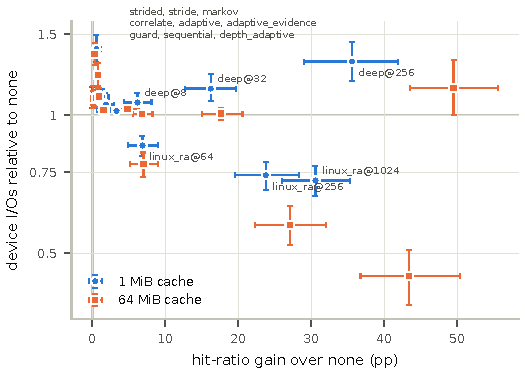
\includegraphics[width=\columnwidth]{figures/f3_device_io_vs_hit}
\caption{Simulated hit-ratio gain over \texttt{none} against device I/Os
relative to \texttt{none}, C1, both cache sizes, with paired \ciLevel{}
bootstrap intervals over the \diskTraces{} traces. Only window growth lies below
one.}
\label{fig:f3}
\end{figure}

\textbf{The learned class router.} The classifier-routed \texttt{adaptive}
policy is \decDiskPOneAdaptiveAssumedOneMiBVerdict{} than \texttt{sequential} at
both capacities (P1): \decDiskPOneAdaptiveAssumedOneMiBPairedCI{} paired and
\decDiskPOneAdaptiveAssumedOneMiBClusterCI{} cluster at 1\,MiB, losing on
\diskDeltaHitRatioAdaptiveVsSequentialOneMiBLosses{} of
\diskDeltaHitRatioAdaptiveVsSequentialOneMiBN{} traces, and
\decDiskPOneAdaptiveAssumedSixtyFourMiBPairedCI{} at 64\,MiB (losing on
\diskDeltaHitRatioAdaptiveVsSequentialSixtyFourMiBLosses). It still beats
\texttt{none} (\diskVsNoneAdaptiveOneMiBCI), but by less than the two-block
read-ahead it routes between, and with more device I/Os
(\diskIORatioAdaptiveOneMiB).

\textbf{The feedback gate.} Against \texttt{sequential}, \texttt{guard} is
\decDiskPTwoGuardAssumedSixtyFourMiBVerdict{} at 64\,MiB
(\decDiskPTwoGuardAssumedSixtyFourMiBPairedCI) and at 1\,MiB its result is
``\decDiskPTwoGuardAssumedOneMiBVerdict'' (paired
\decDiskPTwoGuardAssumedOneMiBPairedCI, cluster
\decDiskPTwoGuardAssumedOneMiBClusterCI). At the break-even cost model it is
\decDiskPTwoGuardBreakEvenOneMiBVerdict{} at both capacities and stays within
\diskBreakEvenVsNoneGuardOneMiB{} of \texttt{none}. The gate limits waste and device
work (\diskIORatioGuardOneMiB{} of \texttt{none}'s I/Os, against
\diskIORatioSequentialOneMiB{} for \texttt{sequential}) but adds no hits over
\texttt{sequential}.

\textbf{Which lever is smallest.} The pre-registered ordering compares the
intervals of $|\Delta|$ against \texttt{sequential}. At 1\,MiB the predictor
(\decDiskOneMiBPredictorSmallestPredictorPairedCI{} pp paired) and the
feedback gate (\decDiskOneMiBPredictorSmallestFeedbackPairedCI) cannot be
ordered; both are smaller than depth
(\decDiskOneMiBPredictorSmallestDepthPairedCI) and window growth
(\decDiskOneMiBPredictorSmallestWindowGrowthPairedCI), and depth is smaller than
window growth, in both the paired and the cluster intervals. At 64\,MiB the
order is complete: feedback, then the predictor, then depth, then window
growth. So the rule's verdict at both capacities is that
\decDiskSixtyFourMiBPredictorSmallestVerdict: the learned predictor moves the
hit ratio little, but the feedback gate moves it as little or less.

\textbf{Robustness.} Of the \decTallyCThree{} P1--P4 decisions that C3 repeats,
\decTallyCThreeRobust{} are \emph{robust} on a second slice of the subset traces;
\texttt{deep@32} against \texttt{none} is
\decDiskCThreeDeepAtThirtyTwoAssumedVerdict{} (better on the first slice,
paired-only on the second). On FIU, \decTallyCFourCapInsensitive{} of
\decTallyCFour{} are cap-insensitive between merge caps of 256 and 1024
sectors. Request reconstruction matters a great deal: on FIU at C2,
\texttt{deep@8} gains \diskDeltaFiuCTwoHitRatioDeepAtEightVsNoneOneMiBCI{} on merged
requests but \diskDeltaFiuCTwoNoneHitRatioDeepAtEightVsNoneOneMiBCI{} on the unmerged
4\,KiB page records, an artefact of counting each page as a request that we
report only as a sensitivity view.

\textbf{Learned depth and the LSTM.} The GPU-trained depth controller is
\decDiskLearnedDepthVsVcfCapTwoHundredFiftySixVerdict{} than the
validation-chosen fixed depth at both action caps, on held-out test segments:
\decDiskLearnedDepthVsVcfCapSixtyFourPairedCI{} with a 64-block cap (cluster
\decDiskLearnedDepthVsVcfCapSixtyFourClusterCI; it wins on
\ldVsVcfCapSixtyFourWins{} of \ldVsVcfCapSixtyFourN{} traces) and
\decDiskLearnedDepthVsVcfCapTwoHundredFiftySixPairedCI{} with a 256-block cap,
over \ldSeedsCapTwoHundredFiftySix{} seeds. The GPU study records prefetches,
not device I/Os: the controller issues \ldIssuedVsVcfCapSixtyFour{} and
\ldIssuedVsVcfCapTwoHundredFiftySix{} as many as VCF under the two caps. It does beat \texttt{deep@8}
(exploratory; \ldVsDeepEightCapTwoHundredFiftySixCI), but \texttt{deep@8} is not the fair
baseline: the depth a validation split chooses is. The LSTM predicts address deltas, so we compare only its
cache outcome: on its \lstmTraces{} traces its mean test hit ratio
(\lstmMeanHit) is below \texttt{linux\_ra}'s (\lstmMeanLinuxRaHit) on
\lstmBelowLinuxRa{} of \lstmTraces{} and close to \texttt{none}'s
(\lstmMeanNoneHit); its contended GPU timings are not quoted.

% VII. Real-device validation (measured). Every number is labelled measured
% with its device, think-time model and host load. Prediction error and
% k_eff are stated per trace and per think model, never as a property of
% HDDs or SSDs (constraint 15).
% Feeds from: results/realio/realio.csv, realio_summary.csv,
% device_*.json and provenance.json (E3).
% Generated: table T3; figure F5.

\section{Real-Device Validation}\label{sec:realio}

\todo{Table T3: backend by mode by think time with hit ratio, full-hit
fraction, mean, p50 and p99 latency, late hits, device MiB and k, from
results/realio/realio\_summary.csv.}

\todo{Fig. F5: simulated hit ratio versus measured mean latency, closed and
spread think models, HDD and SSD, from results/realio/realio\_summary.csv.}

\todo{The simulator prediction error, the rank correlation and the
kernel\_ra baseline, from results/realio/realio\_summary.csv; the simulator
parity assertion from results/realio/realio.csv.}

% VIII. Web results (simulated). Object sizes, RTT and bandwidth are
% assumed (constraint 8). Headline comparisons are against the best fixed
% depth at the same capacity and against transition top-1 (constraint 7).
% Feeds from: results/web/dataset_profile.json, freshness.csv,
% policy_metrics.csv, comparisons.csv, decomposition.csv, seq_metrics.csv,
% calibration.csv (E4, E5).
% Generated: tables T4, T5, T6; figure F6.

\section{Web Results}\label{sec:web}

\todo{Table T4: the RetailRocket event counts and pair kinds (novel,
self-repeat, revisit), from results/web/dataset\_profile.json.}

\todo{Fig. F6: coverage at K versus index freshness, from
results/web/freshness.csv.}

\todo{Table T5: what moves the needle (freshness, depth, controller,
scorer) with CIs, from results/web/decomposition.csv.}

\todo{Table T6: per-capacity validated comparisons against the best fixed
depth, fixed0 and transition top-1, from results/web/comparisons.csv; the
feedback gate, from results/web/policy\_metrics.csv.}

\todo{The GRU sequence model against counts over seeds, from
results/web/seq\_metrics.csv; a footnote on calibration, from
results/web/calibration.csv.}

% IX. Live HTTP results (measured on loopback with an emulated network;
% RTT, bandwidth and object sizes are ASSUMED; constraint 8). Only valid
% passes are cited, and SSD-store passes with more than 1 % foreign I/O are
% left out (lead ruling; genlib.live_citable).
% Sources: results/live/{live_metrics,live_parity}.csv, live_config.json,
% via numbers.tex and paper/decisions.py. Generated: Table T7 (T7b and
% Fig. F7 in the appendix).

\section{Live HTTP Results (Measured)}\label{sec:live}

% t7_live.tex -- GENERATED by paper/tables/make_tables.py; do not edit.
% Inputs: live/live_metrics.csv, live/live_parity.csv
\begin{table*}[t]
\centering
\footnotesize
\setlength{\tabcolsep}{3pt}
\caption{Live HTTP replay (measured on loopback with an emulated network; RTT, bandwidth and object sizes are ASSUMED). Milliseconds of wait saved per view against the no-prefetch baseline: mean over citable passes (valid, and at most 1\% foreign I/O on the store device), with the envelope of the per-pass 95\% session-bootstrap CIs. Parity: sessions whose live counters differ from the simulator's.}
\label{tab:t7_live}
\begin{tabular}{llrrrrrrrr}
\hline
Store & Policy & Passes & Hit (\%) & Wait (ms) & Saved (ms) & Ideal saved & Wasted KiB & Bytes & Parity \\
\hline
\multicolumn{10}{l}{\emph{hdd object store}} \\
\hline
hdd & adaptive\_0.01 & 3 & $27.3$ & $109.1$ & $4.98$ {\scriptsize [$4.14$, $5.89$]} & $3.19$ & $94.6$ & $2.19\times$ & 0 \\
hdd & adaptive\_0.1@trans\_online & 3 & $29.2$ & $105.8$ & $8.27$ {\scriptsize [$7.09$, $9.73$]} & $6.12$ & $95.4$ & $2.20\times$ & 0 \\
hdd & feedback\_0.01\_eps0.005 & 3 & $27.9$ & $107.1$ & $6.99$ {\scriptsize [$5.95$, $8.19$]} & $4.34$ & $159.4$ & $3.00\times$ & 0 \\
hdd & fixed0 & 3 & $24.9$ & $114.1$ & $0.00$ {\scriptsize [$0.00$, $0.00$]} & $0.00$ & $0.0$ & $1.00\times$ & 0 \\
hdd & fixed4 & 3 & $28.4$ & $105.9$ & $8.18$ {\scriptsize [$6.91$, $9.71$]} & $5.09$ & $455.0$ & $6.71\times$ & 0 \\
hdd & fixed8 & 3 & $27.4$ & $106.9$ & $7.23$ {\scriptsize [$6.33$, $8.14$]} & $3.32$ & $1108.8$ & $14.91\times$ & 0 \\
\hline
\multicolumn{10}{l}{\emph{ssd object store}} \\
\hline
ssd & adaptive\_0.01 & 1 & $27.3$ & $101.8$ & $3.39$ {\scriptsize [$2.75$, $4.13$]} & $3.19$ & $94.6$ & $2.19\times$ & 0 \\
ssd & adaptive\_0.1@trans\_online & 2 & $29.2$ & $98.8$ & $6.36$ {\scriptsize [$5.34$, $7.51$]} & $6.12$ & $95.4$ & $2.20\times$ & 0 \\
ssd & feedback\_0.01\_eps0.005 & 2 & $27.9$ & $100.6$ & $4.58$ {\scriptsize [$3.72$, $5.67$]} & $4.34$ & $159.4$ & $3.00\times$ & 0 \\
ssd & fixed0 & 3 & $24.9$ & $105.2$ & $0.00$ {\scriptsize [$0.00$, $0.00$]} & $0.00$ & $0.0$ & $1.00\times$ & 0 \\
ssd & fixed4 & 3 & $28.4$ & $99.8$ & $5.40$ {\scriptsize [$4.45$, $6.53$]} & $5.09$ & $455.0$ & $6.71\times$ & 0 \\
ssd & fixed8 & 2 & $27.4$ & $101.8$ & $3.39$ {\scriptsize [$2.64$, $4.14$]} & $3.32$ & $1108.8$ & $14.91\times$ & 0 \\
\hline
\end{tabular}
\\[2pt]{\scriptsize 0 headline pass-policy row(s) failed the validity gate and 5 valid row(s) carried more than 1\% foreign I/O on the store device; both are excluded.}
\end{table*}


Every saving here is measured on loopback with an emulated \liveRttMs{} round
trip, a \liveMbps{} link and assumed object sizes; it is not a page-load
speedup of a real site. All \liveRows{} pass--policy rows passed the validity
gate, with \liveParityMismatches{} sessions whose live counters differ from the
simulator's (H1); \liveFlaggedRows{} SSD-store rows had over one percent foreign
I/O and are not cited.

\textbf{Prefetching lowered the wait.} With the hard-disk object store, all
\decTallyHTwoHddLowersTheMeanWait{} prefetching policies lowered the mean wait
against no prefetching in every repetition (H2; Table~\ref{tab:t7_live}). The
online-index controller (\polOnline) saved
\liveSavedHddAdaptiveZeroPointOneAtTransOnlineCI{} per view and \texttt{fixed4}
\liveSavedHddFixedFourCI, against a no-prefetch wait of \liveBaseWaitHdd; the
bracket is the envelope of the per-repetition session-bootstrap intervals. On
the SSD store \decTallyHTwoSsdLowersTheMeanWait{} of \decTallyHTwoSsd{}
policies lowered the wait; for \polAdaptive{} the effect is
\decLiveHTwoSsdAdaptiveZeroPointZeroOneVerdict, because only
\liveRepsSsdAdaptiveZeroPointZeroOne{} of its \liveHeadlineReps{} repetitions was
unflagged.

\textbf{The instant-prefetch model understated the hard-disk benefit.} The
model-ideal wait is zero on a hit and the round trip plus transfer on a miss.
On the hard-disk store the measured saving exceeded the model-ideal saving for
all \decTallyHThreeHddTheInstantPrefetchModelUnderstatesTheBenefit{} policies
(H3): \texttt{fixed8} saved \liveSavedHddFixedEight{} against a model-ideal
\liveIdealSavedHddFixedEight. The ideal model has no disk; a plausible reason is that
every demand miss on the hard disk also waits for a seek, which a prefetched
object avoids. On
the SSD store all \decTallyHThreeSsdConsistentWithTheModel{} policies were
consistent with the model, and the store changed the saving for
\decTallyHSevenTheStoreChangesTheDelta{} of \decTallyHSeven{} policies (H7).

\textbf{Bytes, scheduling and hints.} The savings cost bandwidth:
\texttt{fixed8} transferred \liveBytesXHddFixedEight{} the bytes of no
prefetching and saved less than \texttt{fixed4}; the two validated adaptive
controllers moved \liveBytesXHddAdaptiveZeroPointZeroOne{} and
\liveBytesXHddAdaptiveZeroPointOneAtTransOnline, and they are the only policies
no other policy beats on both saved wait and bytes (H4, descriptive;
Fig.~\ref{fig:f7}). Demand priority on the link matters for deep prefetching:
under a FIFO link, \texttt{fixed8}'s change in wait was
\decLiveHFiveSsdFixedEightFIFOCI, against \decLiveHFiveSsdFixedEightPriorityRepOneCI{}
with priority, so \decLiveHFiveSsdFixedEightVerdict{} (H5); for \texttt{fixed4}
there was \decLiveHFiveSsdFixedFourVerdict. Server-side read-ahead hints alone,
with no client prefetch, lowered the wait in one repetition on the hard disk
(H6; \decLiveHSixHddHintFixedEightCI{} for eight hinted objects).

% X. Cross-domain discussion. States how the pre-registered hypothesis came
% out, from the decision rules of each results/*/PREREGISTERED.md
% (paper/decisions.py). Does not generalise from one trace, capacity or cost
% (constraint 7). Generated: Fig. F8 (Table T8 in the appendix).

\section{Cross-Domain Discussion}\label{sec:discussion}

\begin{figure*}[t]
\centering
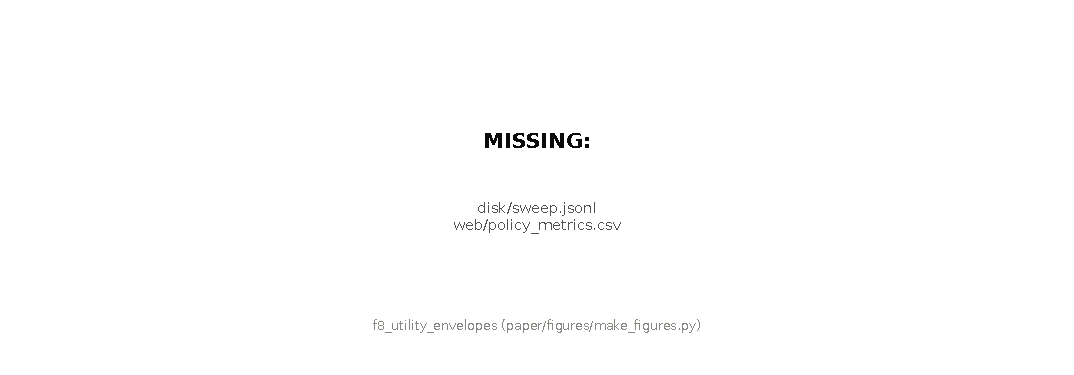
\includegraphics[width=\textwidth]{figures/f8_utility_envelopes}
\caption{Simulated utility $U(c)$ of every policy (grey) and its upper envelope
(coloured by the winning policy) against the cost of one prefetch. Left: disk,
C1, 1\,MiB, means over \diskEnvelopeTracesOneMiB{} paired traces, with the two cost
models marked. Right: web test split, logistic ranker, capacity 8, with the
assumed costs marked. The envelope is computed in hindsight on the test data
and is not a selection.}
\label{fig:f8}
\end{figure*}

\textbf{One objective, two domains.} Fig.~\ref{fig:f8} puts both domains on
the axis of Eq.~\eqref{eq:utility}. On disk, the deepest read-ahead
(\diskEnvelopeBestZeroOneMiB) is best when a prefetch is free, window growth
(\diskEnvelopeBestAssumedOneMiB) at the assumed cost model's $c$, and no
prefetching at the break-even model's $c$ above one. On the web, the best
policy at every marked positive cost is an adaptive controller that chooses
its depth per view (\webEnvelopeBestCostZeroPointZeroOne{} at $c$ =
\webHeadlineCost, \webEnvelopeBestCostZeroPointTwoFive{} at the largest marked
cost). In both domains the policy that wins changes with the price of a
prefetch, and it is a choice of how much to fetch.

\textbf{The hypothesis, by its rules.} The pre-registered hypothesis had three
parts. \emph{The predictor is the smallest lever:} not established in either
study. Every learned predictor lost to its simple, fair baseline (the class
router to \texttt{sequential}, the depth network to the validation-chosen
depth, the logistic ranker to transition counts, the GRU to online counts),
but on disk the feedback gate moved the hit ratio as little or less, and on
the web the GRU's loss could not be separated from the depth lever's gain.
\emph{Depth and freshness are large levers:} supported by the orderings. On
disk, depth and window growth are larger than both the predictor and the gate
at both cache sizes; on the web, freshness is larger than the ranker. \emph{Feedback is a large lever:} not supported. The disk
gate is no better than \texttt{sequential} and the web gate shows no
detectable difference from the adaptive controller; both mainly issue less.
The one gated disk mode above \texttt{sequential}, \texttt{depth\_adaptive},
also chooses its depth (an exploratory comparison).

\textbf{Simulation against measurement.} The two real-system studies point in
opposite directions, and both are measured. On a hard disk with O\_DIRECT and
a closed loop, the simulator's higher hit ratio turned into higher latency in
most cells,
plausibly because prefetch reads compete with demand reads for one device.
Over HTTP, the link serves demand first, a prefetched object skips both the
round trip and the disk, and the instant-prefetch model \emph{understated}
the saving on the hard-disk store.
The simulator's hit ratio is therefore a statement about the cache, not about
latency, and which way the error goes depends on where the bottleneck sits.

\textbf{For a system designer.} Choose how much to prefetch per workload and
per price of a prefetch, prefer window growth that merges reads when device
operations are the cost, keep the statistics fresh, and validate on the real
device before trusting a simulated hit ratio. A learned predictor must beat
these baselines on held-out data to earn its training cost; none of ours did.

% XI. Threats to validity. The full list from MASTER_PLAN section 5; if
% space is short the long form moves to the appendix.

\section{Threats to Validity}\label{sec:threats}

\todo{Trace format: oracleGeneral records carry no read/write flag and no
service time, and timestamps are whole seconds; the FIU page-merge rule is
ambiguous; the request caps (checked by C3); twin traces.}

\todo{Model assumptions: instant prefetch in both simulators (bounded by
the real-device and live HTTP runs); the multi-gen LRU in the kernel versus
LRU in the simulators; assumed web object sizes, RTT and bandwidth; the
per-session cache scope; heuristic thirty-minute sessions; a single
retailer; ranking metrics versus cache utility.}

\todo{Measurement environment: a shared host and a shared GPU, with the
load and contention recorded in each provenance.json.}

% XII. Conclusion and future work. Restates only results already given,
% through the same numbers.tex macros.

\section{Conclusion and Future Work}\label{sec:conclusion}

\todo{What the measurements say about depth, feedback and freshness versus
the learned predictor, in both domains.}

\todo{Future work.}


\bibliographystyle{IEEEtran}
\bibliography{refs}

% MASTER_PLAN L4: the target is 8 pages including figures, references
% extra. Material that does not fit goes after the references; the
% students may cut it.
\appendices
% Appendix (after the references; MASTER_PLAN L4). Holds the material cut
% from the page budget, in the section-5 priority order: T4, F4, F6, F7,
% T8, the FIU merge sensitivity and the full threats list.

\section{Supplementary Results}\label{app:supplementary}

\todo{Whatever does not fit the page budget once WP14 has written the main
sections.}


\end{document}
